\documentclass[journal=jacsat,manuscript=article]{achemso}
%Image-related packages
\usepackage{graphicx}
\usepackage{subcaption}
\usepackage[export]{adjustbox}
\usepackage{wrapfig}

%%\listfiles

\newcommand*\mycommand[1]{\texttt{\emph{#1}}}

\author{Nayanika Das}
\affiliation[UVicUCC]{Computational Biochemistry and Biophysics Lab, Research Group on Bioinformatics and Bioimaging (BI$^2$), Department of Biosciences, Universitat de Vic - Universitat Central de Catalunya, 08500 Vic, Spain}
\author{Vijay Baladhye}
\affiliation[SPPU]{Savitribai Phule Pune University, Pune, India}
\author{Jordi Villà-Freixa}
\email{jordi.villa@uvic.cat}
\affiliation[UVicUCC]{Computational Biochemistry and Biophysics Lab, Research Group on Bioinformatics and Bioimaging (BI$^2$), Department of Biosciences, Universitat de Vic - Universitat Central de Catalunya, 08500 Vic, Spain}
\alsoaffiliation{IRIS-CC}

\title[Evolutionary trends of GPX6 $\Delta G^{\ddagger}$]
  {Computational Free Energy Directed Evolution In Enzyme Design: Exploring Mutational Pathways With Lower Activation Penalty in Glutathione Peroxidase 6 Homologs}

\abbreviations{IR,NMR,UV}
\keywords{Ancestral enzyme reconstruction, enzyme design, empirical valence bond, free energy calculations}

\begin{document}
\maketitle 

\begin{abstract}
Outstanding success in computational protein design has been achieved in recent years by combining machine learning approaches with physicochemical properties analysis of the explored variants. Despite these efforts, however, less success has been obtained in designing good computational protocols for optimization of the enzyme activity. Here we propose the use of the Empirical Valence Bond method to evaluate free energies of activation of the enzyme variants to obtain reasonable mutational pathways leading to a functionally optimized protein. In particular, we propose a method that explores a lower free energy difference pathway for the directed evolution of enzymes based on the EVB activation free energies. To test the idea, we study the hypothetical connectivity of the selenocysteine-containing human glutathione peroxidase 6 protein (GPX6) into its ortholog cysteine-containing mouse GPX6. We show how it is possible to find a mutational pathway connecting the two protein sequences and structures that provide the empirical barriers for the first step of the GPX6-catalyzed reaction. Moreover, this protocol offers the potential for addressing complex issues such as epistasis in enzyme engineering, further enhancing its utility in enzyme optimization.
\end{abstract}

\section{Introduction}

Selenium (Se), in the form of selenocysteine (Sec, U—the 21st amino acid) occurs in 25 proteins in the human proteome. Insertion of Sec into a protein is much more complicated than the other 20 amino acids because a UGA stop codon must be recoded as a sense codon for Sec \cite{Hondal2011}. The complexity of this process signifies that Sec must fulfill a chemical function that exerts biological pressure on the genome to maintain the Sec-insertion machinery \cite{Hondal2011}. This view also implies that since Se “speeds reactions” Sec should have widely substituted for Cys in enzymes, which clearly has not occurred. Specific reasons for the usage of Sec might include the enhanced nucleophilic character of Se relative to S, or another might be the much lower pKa of a selenol relative to that of a thiol \cite{Hondal2011}. GPXCys-containing proteins act on alternative substrates for peroxidation and may have additional functions, including signaling and oxidative protein folding. Thus, all GPX proteins may protect cells from oxidative stress \cite{Rees2024}. 

\subsection{Mechanism of GPX}

A catalytic mechanism proposed for GPX3 by Morokuma et al. based on DFT calculations has the resting state of Sec as selenol as shown in the figure below. Morokuma \cite{Prabhakar2006} performed ONIOM(QM:MM) calculations to assess the effect of protein surroundings on reaction energetics. In the first step, selenolate formation occurs through proton transfer, leading to an intermediate (III) \cite{Prabhakar2006}. The barrier for selenolate formation is 16.4 kcal/mol, and for selenenic acid formation (E-Se-OH), 18.0 kcal/mol \cite{Prabhakar2006}.

\begin{figure}[h]
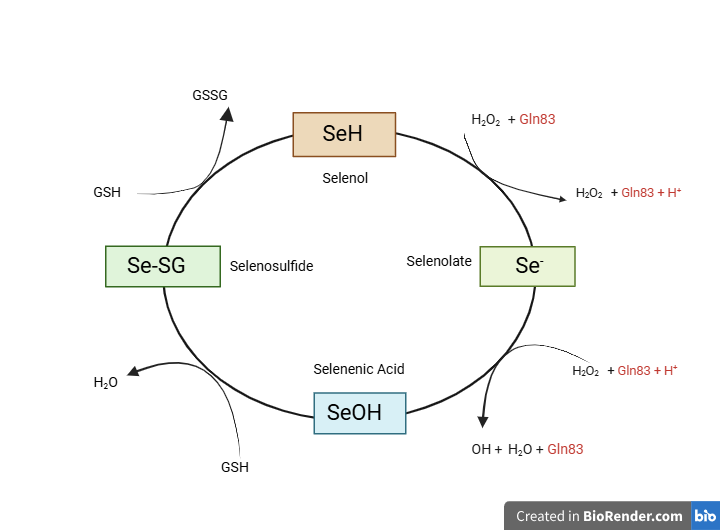
\includegraphics[width=0.7\textwidth, inner]{figures/Catalytic_cycle.png}
\caption{Catalytic Cycle of GPX as given by Morokuma et al., with Se in the resting state as selenol.}
\label{fig:figure1}
\end{figure}

\begin{wrapfigure}{h}{0.7\textwidth}
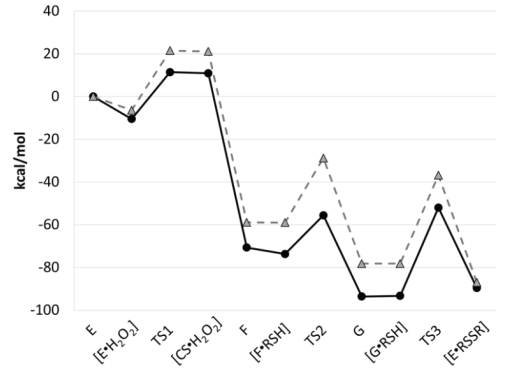
\includegraphics[width=0.7\linewidth]{figures/flohe_energyprofile.png} 
\caption{DFT-calculated energetic profile of the oxidation cycle for SecGPX and Cys analogs.}
\label{fig:figure2}
\end{wrapfigure}

\subsection{Empirical Valence Bond Model based on QM/MM Calculations}

The hybrid QM/MM-based Empirical Valence Bond (EVB) method effectively models activation parameters in enzymatic reactions by constructing potential energy surfaces \cite{Oanca2024}. The EVB Hamiltonian used for activation free energy is as follows:

\[ 
  \left[ {\begin{array}{cc}
    H_{11} & H_{12} \\
    H_{21} & H_{22} \\
  \end{array} } \right]
\]
Here, $ H_{11} $ and $ H_{22} $ are energies of two valence states, and the off-diagonal element $H_{12}$ represents coupling between them. Calibration of EVB parameters—such as the coupling term—is achieved through reference reactions, enabling accurate predictions of activation parameters \cite{Oanca2023}.

\subsection{The Concept of Epistasis and Protein Sequence}

Protein evolution involves trajectories through sequence space influenced by mutation, drift, and selection. Epistasis can cause the effect of mutations to vary in homologs, underscoring the sequence topology’s role in guiding evolution \cite{Starr2016}. Here, we examine epistatic effects in GPX6 homologs (human selenocysteine vs. mouse cysteine) by mutating active-site residues, exploring activation free energy shifts in response to proximal and distal mutations.

\begin{figure}
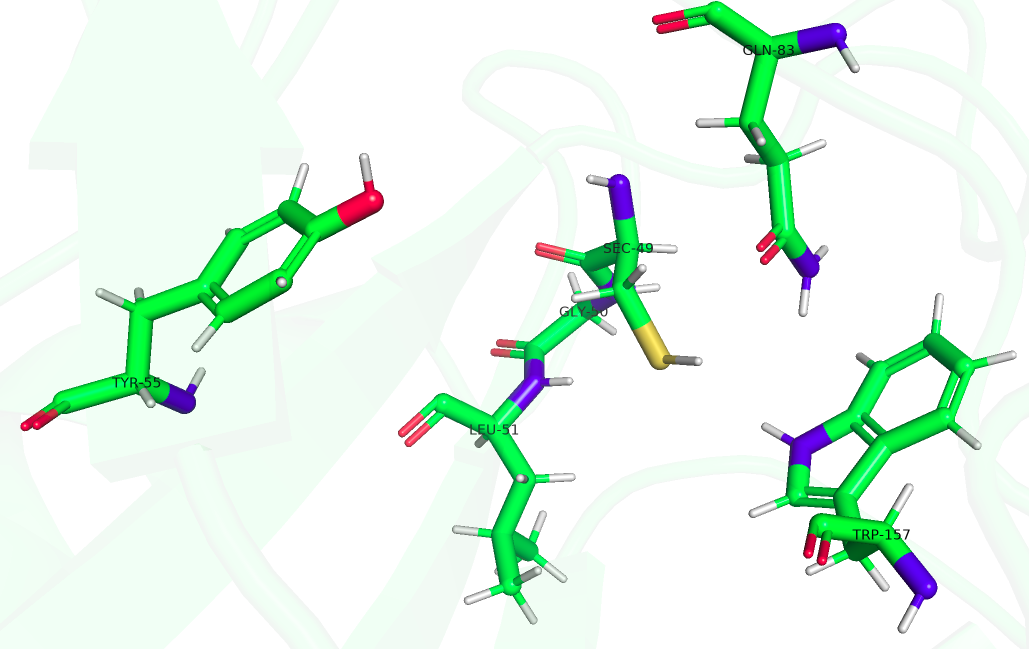
\includegraphics[width=0.7\linewidth]{figures/activesite_humansec.png} 
\caption{Active Site of Human GPX6}
\label{fig:figure4}
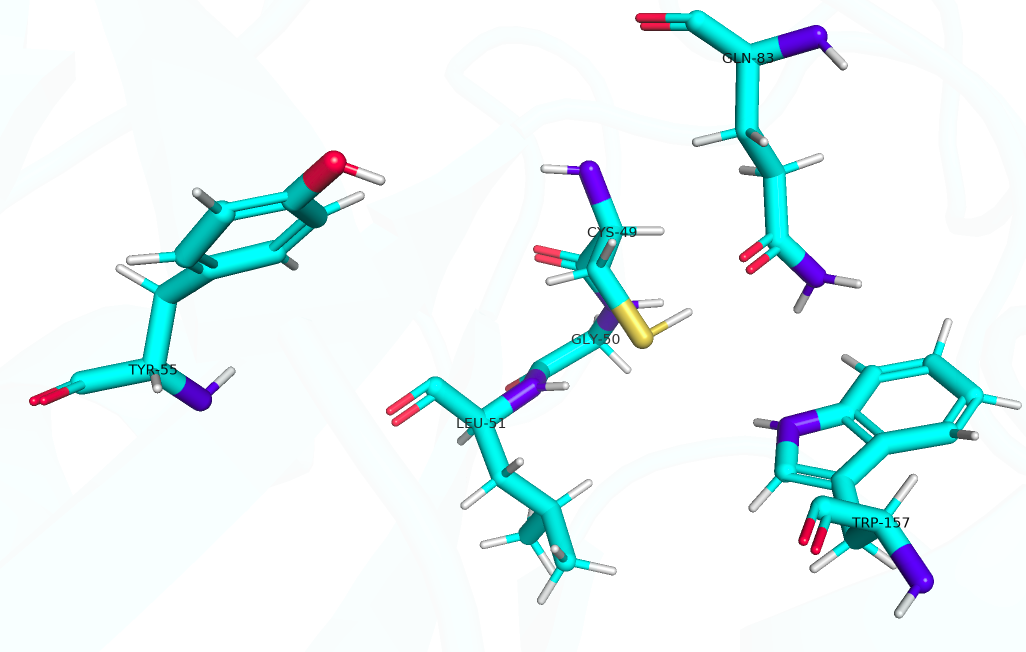
\includegraphics[width=0.7\linewidth]{figures/activesite_mousecys.png} 
\caption{Active Site of Mouse GPX6}
\label{fig:figure5}
\end{figure}

\section{Selection of Variants}

A multiple sequence alignment (MSA) between human and mouse GPX6 sequences identified 47 distinct positions as candidates for mutagenesis. Distances from Cys/Sec49 were grouped into bins (<10 Å, 10-15 Å, etc.) to facilitate mutational impact analysis relative to the active site. Gradual mutations from proximal to distal residues allowed for examining incremental effects on activation barriers.

\section{Computational Model Preparation}

The initial structure for mouse Cys WT was derived from PDB ID 7FC2; the human Sec WT was generated with AlphaFold. Missing force field parameters, including selenol (U) parameters, were prepared in Maestro’s FFLD. The Q program was used for simulations with TIP3P water.

\subsection{Free Energy Calculation Using Q}

Free energy perturbation (FEP) calculations in Q employ consecutive input files with mapping parameters ($\lambda$ values) from [1,0] to [0,1] between states. The Qfep program computes total $\Delta G$ from the initial to final states:

\begin{equation}
    \Delta G = \sum \Delta g = \sum -R \cdot T \cdot \ln \left\langle e^{-\left(\frac{\Delta V_{\text{eff}}}{R \cdot T}\right)} \right\rangle_{A}
\end{equation}

\end{document}
